\chapter{Problem Analysis}
This chapter will strive to answer the research questions posed in \ref{sub:ResearchQ} and any other relevant information that arrises. 


\section{Research}
This section focuses on the research necessary for the basic understanding of the subject. \todo{write some more} 
\subsection{Effects}
Many voice effects exist today. Some effects are used in most music, and some are not. The effects can be really subtle, or really noticeable.
In this section, common effects will be explained.


\subsubsection{Delay}

A delay effect creates a repetition of the original sound after a period of time\citep{Loeffler_2014}. By using the delay effect, it is possible to simulate the sound of the echo created when yelling into a cave or over a canyon, among a lot of other things.

\subsubsection{Reverberation}

When sound reflects off surfaces in a confined space, its called natural reverberation\citep{Redmon_1997}. Reverberation like this works best when the sound hits hard surfaces. For example, the sound effect that comes when you sing or yell in a church, is reverberation. The sound bounces all around the church hard walls.
Digitally, the way to simulate reverberation is to use a multitude of delays and feedback. This then creates a series of echoes that then slowly decays.

\subsubsection{Pitch Shift}

The frequency of a harmonic sound is called its pitch\citep{Katjaas_00}. By shifting the pitch, the sound will effectively deeper or higher. An example of this is the voice that anonymous people get when they want to hide their voice, this is a lowered pitch. Another example is the “chipmunk voice”, which is achieved through a raised pitch.
Pitch shifting is done by using time-stretching and up- or down-sampling. For example, a time-stretched and down-sampled sound results in a raised pitch.\\

Pitch shifting is also used to create the harmonizer effect. It takes the input voice and shifts its pitch a bit, and then adds it as an additional voice. This can effectively simulate a choir.

\subsubsection{Auto-Tune}

The Auto-tune effect corrects a singer's voice to the correct tone\citep{Hadhazy_2010}. This can be really subtle or plainly obvious. Firstly, the user chooses a reference of scales or tones, and secondly the amount correction to be made.

\subsubsection{Vocoder}

The Vocoder effect combines a singer's voice with another sound - that could be the sound from an instrument or a synthesizer\citep{Vocoder_00}. 
The effect can make the voice sound like a robot. The vocoder needs two inputs, the voice and the instrument. The fundamental frequencies of the voice are converted to levels of amplitude on a series of band pass filters, which then are passed through the instrument sound.

\todo{finish this section with a short summary/conclusion.}
\subsection{State of the Art}
To understand and avoid issues a study of the state of the art on this area was conducted. There is a focus on commercial artifacts based on real-time alterations. \todo{any comments on this intro?}
%Intro to state of the art

\subsubsection{TC Helicon Perform V}

The TC Helicon - Perform V is a simple pedal that attaches to a microphone stand, as seen in figure \ref{tchelicon}\citep{TC}. It has three effect buttons, three preset buttons, a big knob, and other buttons. The pedal effects are reverb, echo, “double” (harmonizer), EQ, compressor, and many more. It is possible to download an app that can connect with the Perform V. The application has many pre-made sounds, and it has a wireless connection. \\

\begin{minipage}{\linewidth}% to keep image and caption on one page
\makebox[\linewidth]{%        to center the image
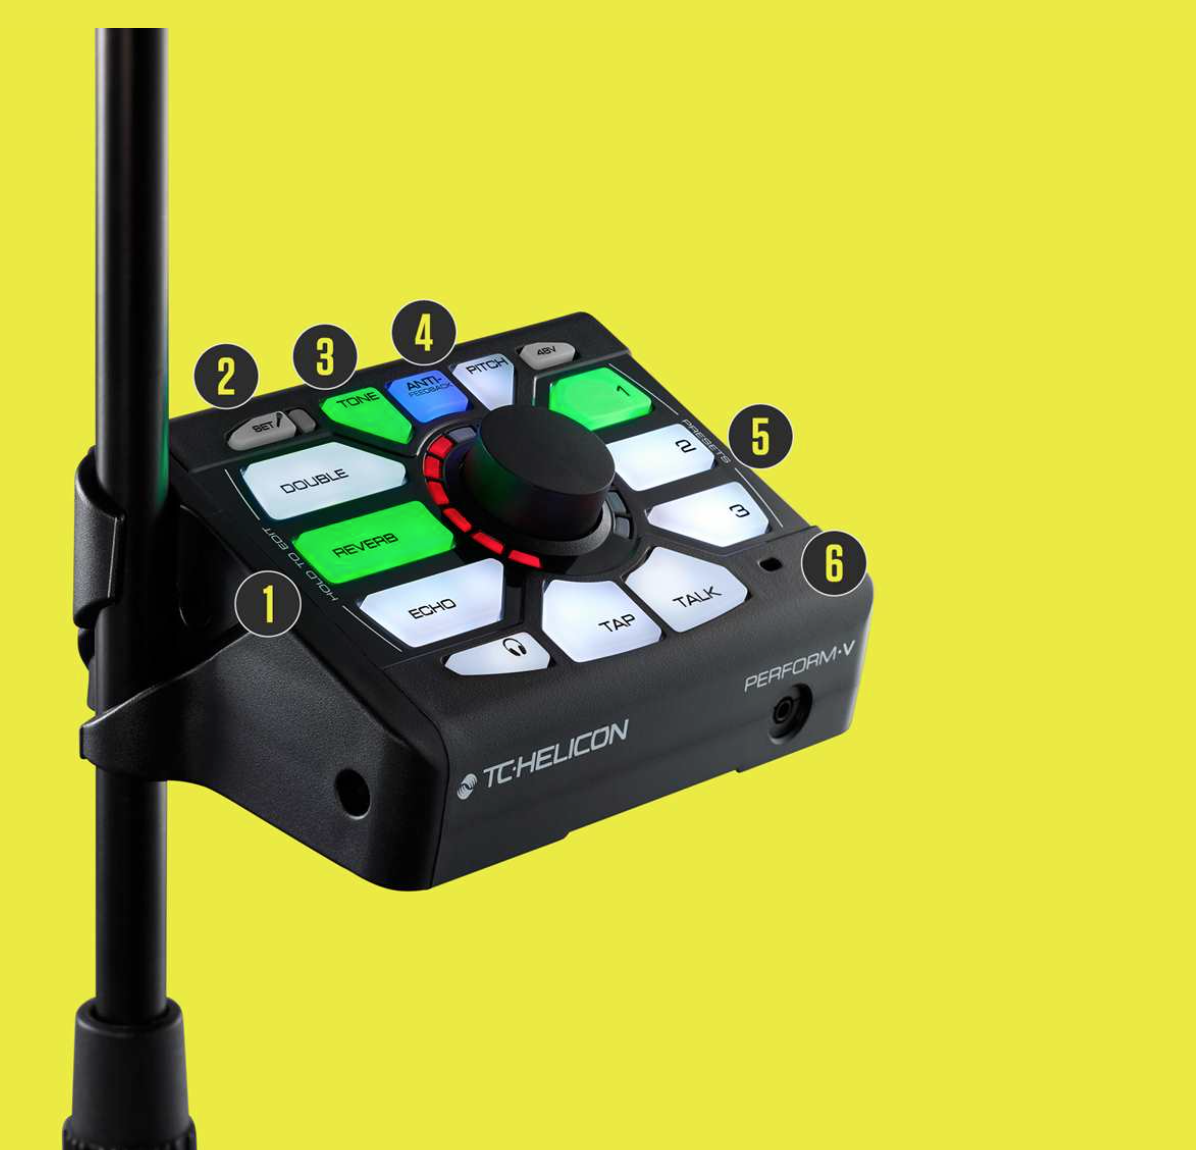
\includegraphics[keepaspectratio=true,scale=0.4]{tchelicon}}
\captionof{figure}{TC Helicon\citep{TC}}\label{tchelicon}
\end{minipage}\\

The Perform V is good for live performing if the singer has the pedal in front of them, on the microphone stand. Preset buttons make it easy to change effect quickly. 
If the singer plays an instrument, it is probably difficult to change effects without interrupting the instrument playing. Another downside is that singer limited to only three presets, and only one knob to turn.

\subsubsection{Electro Harmonix Voice Box}

The Electro Harmonix Voice Box is a more advanced pedal than the TC Helicon\citep{VoiceBox}. It has six knobs: blend, two reverb knobs, “gender bender”, voice mix, and “Mode”, as seen in figure \ref{voice_box}. It has nine different modes, which includes different kinds of harmonies, unison-whistle, and a vocoder, which the TC Helicon does not have.\\

\begin{minipage}{\linewidth}% to keep image and caption on one page
\makebox[\linewidth]{%        to center the image
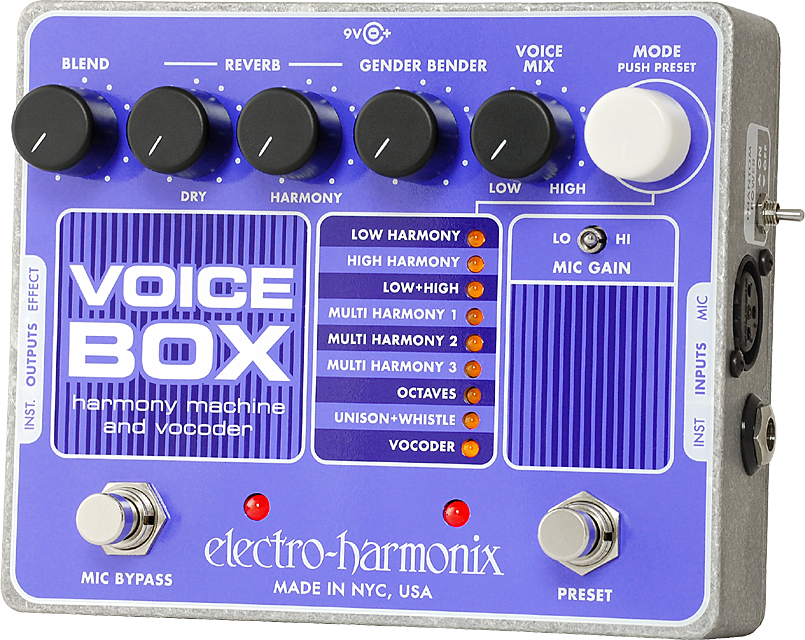
\includegraphics[keepaspectratio=true,scale=0.4]{voice_box}}
\captionof{figure}{Electro Harmonix Voice Box\citep{VoiceBox}}\label{voice_box}
\end{minipage}\\

The Voice Box has to be on a flat surface, like the floor or a table. It is possible to insert an instrument to the pedal, so it can be used for the vocoder. The Voice Box has many effects and knobs - this can make changing effects and effect parameters difficult, even more if the pedal is on the floor.

\subsubsection{Mi.Mu Gloves}

The Mi.Mu Gloves are gloves made for making music, and controlling sound\citep{Mimu}. They are made by scientists, musicians, and artists, and have been in development since 2010. They are wearable, and can be used by one or both hands(see figure mimu). The gloves have been through many iterations, and they are open source. The gloves use gestures, hand and finger movement, finger placement, and other features to control sounds and effects. The hardware includes an ArduImu, flex/bend sensors, accelerometer, gyroscope, haptic motors, LED's, WiFi compatibility, and provides other capabilities.\\

\begin{minipage}{\linewidth}% to keep image and caption on one page
\makebox[\linewidth]{%        to center the image
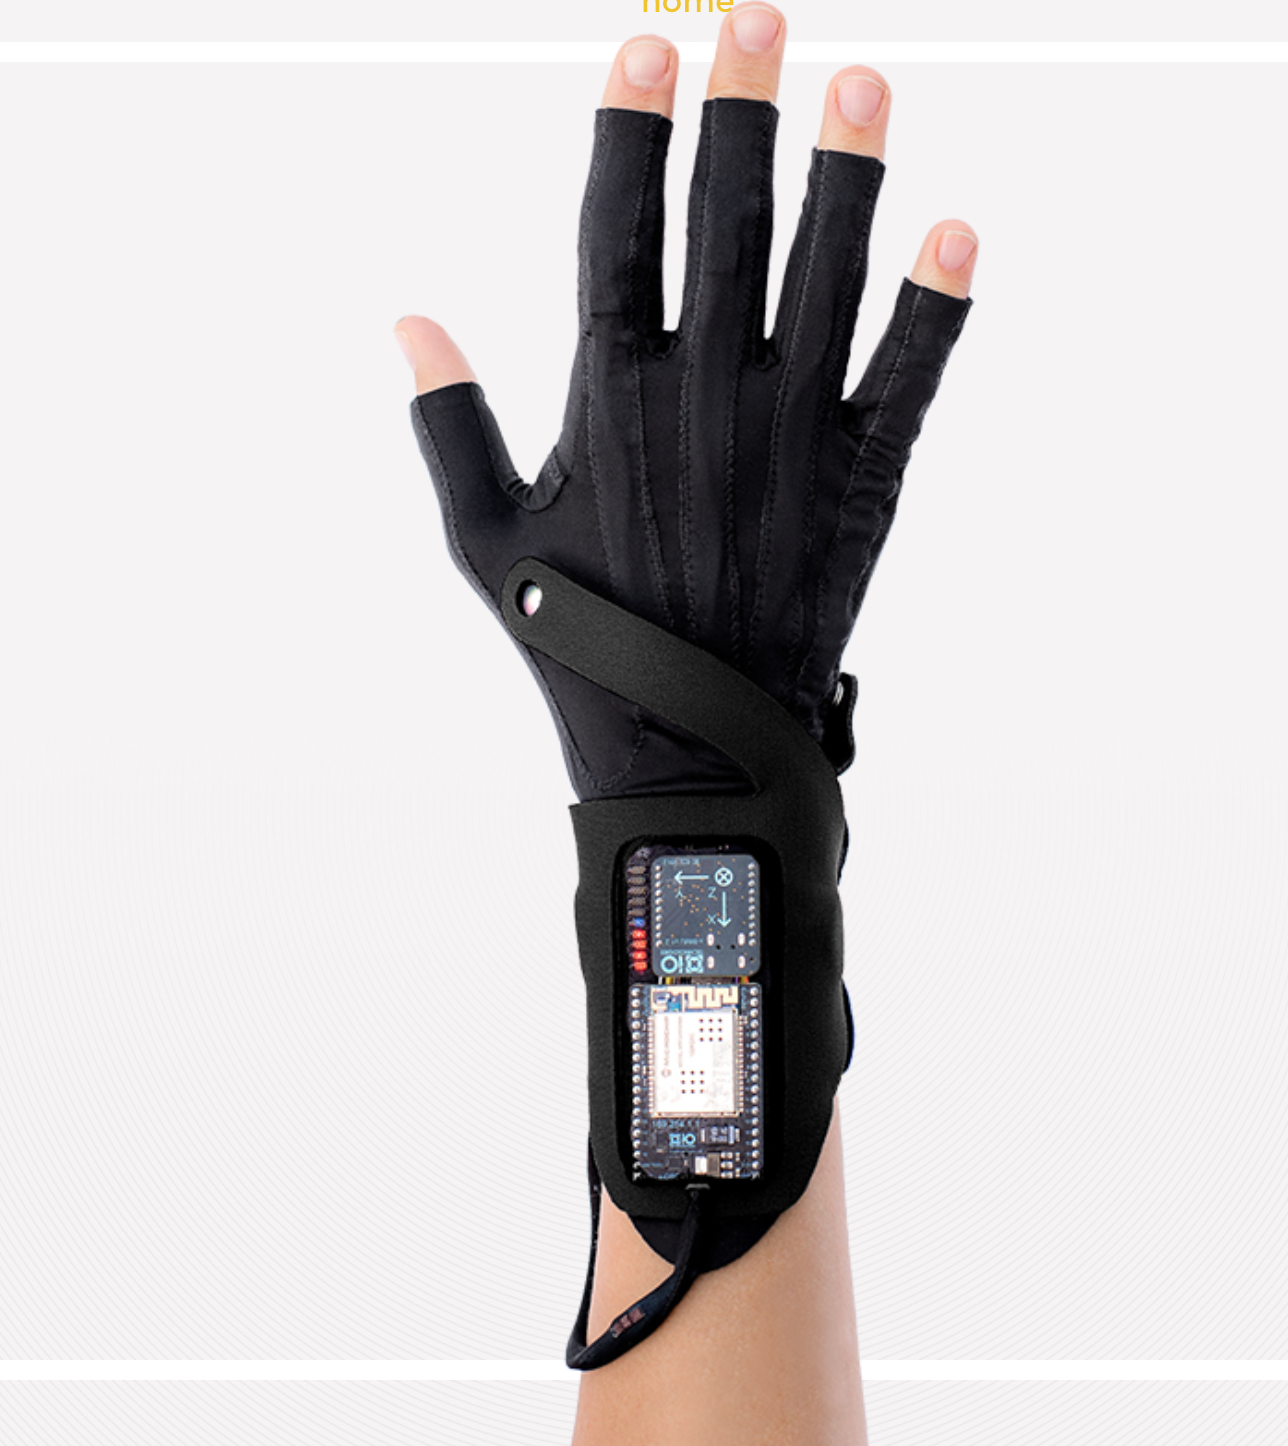
\includegraphics[keepaspectratio=true,scale=0.4]{mimu}}
\captionof{figure}{Mi.Mu Gloves\citep{Mimu}}\label{mimu}
\end{minipage}\\

The gloves are bluetooth or Wi-Fi connected, so the person using the gloves are free to move around, and does not have to worry about wires. They are also battery powered. It is possible to pre-order a pair of Mi.Mu gloves for £5,000, or one glove for £2,500. 
Since the gloves are open source, you can make your own - many different gloves exist - some are simple, and some are complex.

\todo{conclusion/summary here} 

\section{Problem Statement}


\section{Minimum Implementation}
\begin{itemize}
	\item The design must implement the use of an Arduino
	\item The design must implement the use of sensors applicable to the Arduino
	\item The design must implement audio processing
	\item The design must get audio from a microphone
\end{itemize}

